\chapter{Implementation PUT IN OWN FILE}

\section{User interface}
\label{mainimp}
The main display represents the general interface is displayed to the user. This is where the algorithms visual representation will be presented, as well as providing the location of the user interaction elements enabling modification of the algorithms parameters. This interface is a result of the contents of the DisplayFrame Class and its contents. The design for this view is almost as described in section \ref{ssec:mainUI}, appendix B, however, there has been a slight modification to this proposed design.

\begin{figure}[H]
\centering
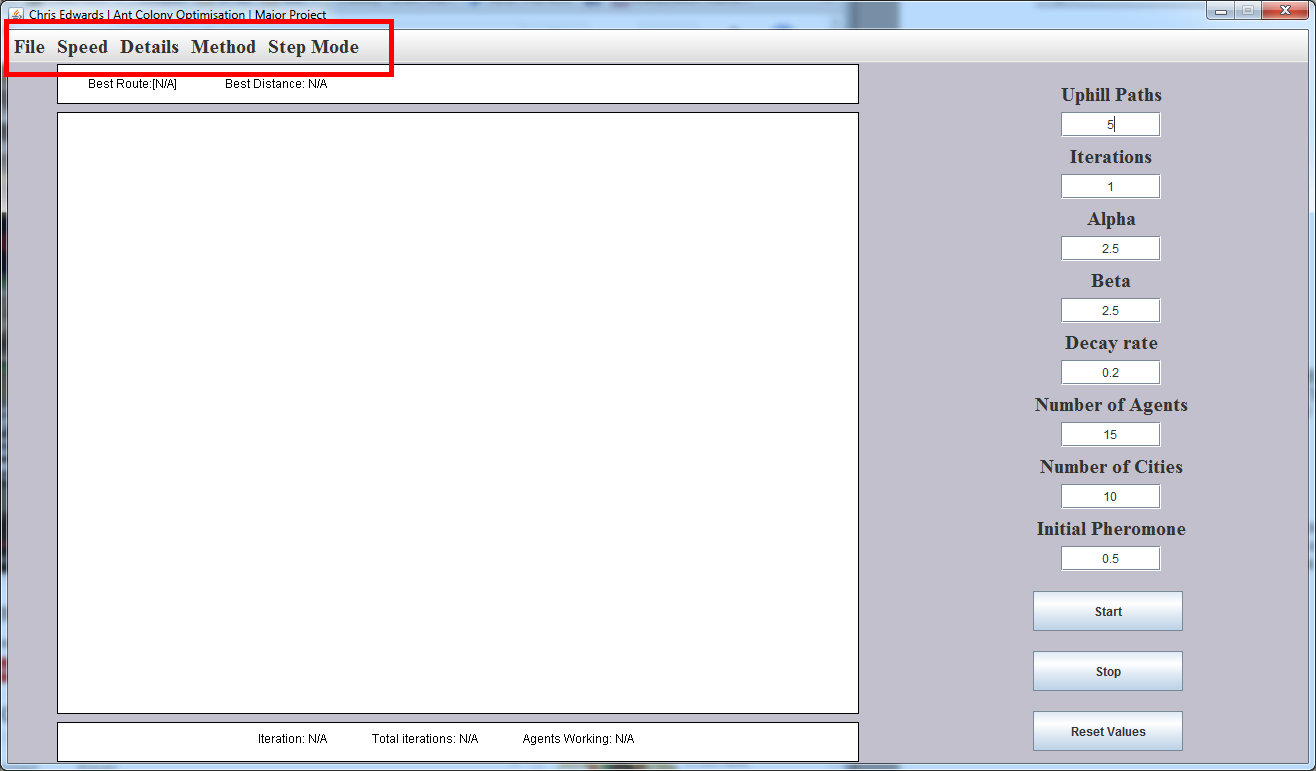
\includegraphics[scale=0.35]{Images/chapter4/displayFrame}
\caption{Implementation of the proposed user interface. The contents of the red polygon highlights the additional features not present in the initial design.}
\label{fig:displayFrameImp}
\end{figure}

The additional features highlighted by the red polygon in figure \ref{fig:displayFrameImp} represent the features which were not initially designed. These features are represented in a separate location to the control panel (right hand side of figure \ref{fig:displayFrameImp}) as there is no logical connection between the menu bar features, and the modification of the algorithm parameters. The author opted to use a menu bar to control the access to these features as the vast majority of users will recognise what a menu bar is, and understand how to interact with such elements. 

The different elements contained in this menu bar relate to general system interactions. The File option enables the user to either load, or save a configuration to a specified file. The Speed option enables the user to change the Thread speed, which will directly change the algorithms rate of execution. The Details menu is used to control access to any additional views. The views which can be access here are; the Uphill Viewer (section \ref{uphillview}), The City Detail View (section \ref{deetzlview}) and the Equation Viewer (section \ref{eqnlview}). In addition to the access of these extra views, the Detail menu also enables the user to disable and enable uphill routes \Large REFERENCE UPHILL ROUTES GENERATION ALGORITHM PSEUDO CODE \normalsize to be generated for current problem. The Method option enables the user to select the current algorithm type from a list of implement algorithm types. Currently the author has implemented a Basic Ant System and an Elitist Ant system so the user can switch between these algorithm types. The Step Mode menu enables the user to enable or disable the step mode functionality. When enabled, step mode will allow the user to step through the algorithms execution at their own pace without the application automatically solving the problem.

\section{Data Structures}

\subsection{Pheromone and Distance Matracies}

\subsubsection{Pheromone}
\label{phero:struct}
A Pheromone Object is used to represent the pheromone concentration for a given edge in the current problem graph, however there is no data stored inside the Pheromone Object which relates this Object to a specific edge. To enable logical indexing of these Objects such that the author could continually the pheromone data for a specific edge is a fairly trivial task however, the method of doing so has changed since the initial proposed design as seen in section \ref{pheroRepsec}, appendix B.

The concept of a using two-dimensional array to store the pheromone data is still present however, the dimensions of such structure are now directly representational of the number of cities present in the current problem. Assume there are $x$ number of cities in the current problem then the length of each array would also become $x$. Therefore the instantiation of the pheromone data structure is of the format $Pheromone[][] pheromone = new Pheromone[x][x]$. Assuming these $x$ cities have the $index$ values $0, 1, ..., x-1, x$ then indexing any edge would be done using the format $pheromone[x][y]$. Given this format, $x$ and $y$ are any valid $City indexes$. For example, to access the pheromone concentration for the edge corresponding to the path from $City\ 0$ to $City\ 5$ would be accessed using $pheromone[0][5]$. As accessing an element in in an array is a $O(1)$ operation this method of access is extremely efficient and supports a problem of almost any size as the data structure resizes with the problem. Figure \ref{initPheroCode}, appendix C represents how the pheromone matrix is initialised using the initial pheromone value for all edges.

\subsubsection{Distance Matrices}

Initially there was no proposed design for the inclusion of data structures representing the distances between each node in the graph as the initial design for the problem representation made it simple to calculate the distance between the current node and the destination node extremely trivial. The author decided that as the problem representation has changed to the TSP there needs to be a better method of accessing the distances between two nodes (Cities).

The design for the distance matrices are based on the implementation provided by Thomas Jungblut \cite{tjung:aco:blog}. The implementation of these data structures is identical to that discussed in section \ref{phero:struct} however, the data stored in each array element represents the $euclideanDistance$ between two $cities$ rather than the pheromone concentration. As defined in section \ref{phero:struct} the size of distance matrices will represent the number of cities. If there are $x$ cities in the current problem then the format for instantiation will be $double[][] distanceMatrix = new double[x][x]$. The way in which elements are accessed also remains the same as above, however once instantiated these values will remain constant as a $City$ cannot move location. These matrices are easily populated after the cities have been instantiated. The code in appendix C figure \ref{initDistanceCode} represents how this has been implemented. A correct implementation would return a distance of $0.0$ if $index[x][x]$ were to be accessed where $x$ is the same value. This is because the distance from any $City$ to itself is 0.
As the probability is represented as $p_{xy}^{k} = \frac{(\tau_{xy}^{\alpha })(\eta _{xy}^{\beta })}{\sum (\tau_{xy}^{\alpha })(\eta _{xy}^{\beta })}$ where $\eta _{xy}$ represents $\frac{1}{distanceMatrix[x][y]}$ (inverted distance). As this function is used extremely often during the algorithms execution rather than converting the value of $distanceMatrix[x][y]$ every time an inverted version is needed it is far more efficient to store an inverted version of the $distanceMatrix$. The code snippet in appendix C, figure \ref{initInverteddistanceCode} demonstrates how this can be implemented. The $invertDouble(distanceMatrix[i][j])$ in said figure simply returns the value of $\frac{1}{distanceMatrix[x][y]}$ however if $distanceMatrix[i][j]\ ==\ 0.0$ then $0.0$ is returned as $\frac{0}{distanceMatrix[x][y]}$ is illegal.
  
\subsection{Agent and City Collections}

Both Agent and City Objects are designed to be stored using data structures which implement the List$<$type$>$ Java interface. As the number of Cities and Agents present in the current problem is dynamic and user defined the size of the data structure must be established at runtime and therefore the data structure chosen must scale well and maintain performance regardless of its size. In addition to this, a user is able to modify the amount of Agents and Cties once created, therefore the data structure must be able to be effectively resized dynamically without complication. The ArrayList data structure has been chose to store the Agents and Cities as it is scalable and can be dynamically resized. An Array implementation could be used here however, if the Array reached capacity then there would need to be conditionals put in place by the author to copy the contents of the full Array into a new, larger Array instance. The use of ArrayList means that the author does not have to worry about these conditionals are they are handled for the author by the ArrayList implementation. In addition to this, the order the elements in generally unimportant, accessing a random index however is. Using an ArrayList provides $O(1)$ random element access using the provided $get(index)$ method. Also inserting into an ArrayList is $O(1)$ where as an Array implementation would provide $O(n)$ insertion as the next free index would have to be located. As the ordering in unimportant there is no reason to use a LinkedList data structure and the improved performance of the ArrayList versus an Array has enabled the author to confidently select an ArrayList implementation as the best suited data structure. 

Unless explicitly stated by loading a configuration from a file, the locations of the $City$ elements in collection of cities are randomised. There are conditionals in place to ensure that two cities cannot be placed in the same location as this is a possibility if the locations of such cities is random. The implementation of the $City$ instantiation can be found in appendix C, figure \ref{initCity}.

The starting location of the Ant Objects represented as elements in the collection of agents is also randomised. This random value is however limited to a range of integers with a maximum possible value equal to $cities.size() - 1$. As indexes start at 0, this enables the random function to return any $City$ index such that it is possible for an agent to start at any $City$ location. The implementation of this agent instantiation is defined in appendix C, figure \ref{initAnt}.

\subsection{Best Route representation}

Storing the current best route is slightly more complicated than storing the collection of Agents or Cities as the ordering is important. As the ordering is important the accessing of random indexes is irrelevant as the elements stored in this data structure when parsed in order represent the order to cities which the agent visited in order to produce this best route. The indexing of random elements would enable the elements to be parsed in an incorrect order, thus this functionality will not be used by the author and therefore the data structures performance in executing such task is completely nullified. The data structure used for this representation does not need to have dynamic resizing capabilities as the length of any best route will represent the number of cities in the problem as an agent must visit every City once and only once. The author reduced his choice to using an ArrayList or a LinkedList implementation. A LinkedList implementation has massive performance enhancements when compated to an ArrayList as a LinkedList can provide constant time ($O(1)$) insertion and deletion operations using iterators which can be relied upon regardless of the magnitude of such data structure in combination with the lack of regard to element ordering. An ArrayList cannot reliably provide such performance. This in addition to the fact that the ordering of elements is important, has lead the author to decide on using a LinkedList data structure for the representation of the best routes.

\section{Pheromone Operations}

The translation of the pseudo-code described in algorithm \ref{aco:pseudo:pherofunc} was a fairly simple process as the pheromone algorithm is itself relatively simple. Once implemented the author quickly realised that the pheromone operations (deposit and decay) were not behaving correctly. During the course of agents $move()$ method every time the agent moves from its current location to its next location pheromone proportional the distance travelled would be deposited on the corresponding edge. The problem was that every time this pheromone was deposited the global pheromone was in fact being decayed so the global pheromone was being decayed every time the agent moved. In order to prevent this problem from arising rather than directly updating the pheromone on the edge when the ant moves the agents pheromone deposit on this edge is instead added to a secondary $newPhero$ variable in the Pheromone Object for this corresponding edge. This variable is used to collate the total amount of new pheromone to be deposited for any edge. When it is time to update the edge pheromone, every Pheromone Object is iterated through and value present in this $newPhero$ variable is used in the pheromone calculation allowing for correct behaviours to be represented. This is slightly more complicated than the author envisioned however, the additional complexity is essential to ensure correct behaviour. The implementation of this method is shown in appendix C, figure \ref{codephero}.

\section{Solving the Problem}

The author encountered unforseen complications when implementing the pseudo-code represented in aglorthm \ref{aco:pseudo2}. The subsections below described the problems with the implementation process and their associated solutions.

\subsection{Agent Movement}
\label{antyMove}
The author has problems initially with his implementation of the probability based movement of the agents. The implementation of the Ant's $move()$ function worked as expected there were no complications assoicated with that however, the complication that the author encounted involved the probabilistic selection of the Ant's next location. The problem caused every Ant that started at the same City index to take exactly the same route. Upon debugging the Ants $getNextProbableNode(int y)$ function the author realised that there was in fact no random element assoicate with this method and the City with the highest probability was constantly selected thus, the Ants never had the ability to divert away from the best looking route causing local solutions to be present. The author attempted to implement this random element into his method however the aglorithm did not perform as effeciently as expected. Thomas Jungblut had provided an open source implementation of a basic Ant Colony Optimisation algorithm \cite{tjung:aco:blog}. This implementation was provided free of charge and allowed modification which enabled the author to replace his lackluster node selection function with a the one provided in this working implemention. This node selection function did however require modfication by the author to ensure correct operation with his architecture. Once this method had been modified and implemented the node selection process for the Ant's next location worked as initially intended. The author realised that his implemention took completely the wrong approach which involved sorted the candidates locations based on thier assoicated probability. Had the author not accepted that the re-use of a working implemention is the best way to progress the application then a reduce in project quality would have been a possibility.  The implementation of this node selection method can be seen in appendix C, figure \ref{nextNodeCode}. If this method returns $-1$ then the Ant is deemed to have completed its walk.

\subsection{Automated Solving}
\label{autoSolve}
Implementing an algorithm which once started, executes untill completion was in fact fairly simple to do initally. This simplistic implementation stemmed from the fact that initially the aglorithm only considered the fact there was one iteration. As there was one interation it was simple to define a stop condition which was in fact when every agent had completed its walk which meant the aglorithm stoped when $Ant.getFinished()\ returned\ true$ for every Ant. Once the author had impleted automatic execution for one interation, the ability for a user defined number of interations was implemented. The addition of the to support $x$ number of iterations where$x\ >\ 1$ introduced several new complications. Each new iteration meant that the Ants need to be reset so that they forget everything from the previous iteration(s) but the pheromone levels, Cities and current best route must all be persevered accross iterations. In order for this to be possible, the author adpated to algorithms stop condition to now be relative to the number of iterations or in other words stop when $currentIteration\ ==\ totalIterations$. A new iteration is started when all Ant's have finished thier walk, instead of checking every Ant for the condition $Ant.getFinished()\ ==\ true$ once an ant had finished a variable representing the total number of Ants current working (unfinished) was reduced by 1. When this value reaches 0, there are no Ants currently working thus the iteration has completed. Once an iteration has completed the Ants must be reset so the next iteration can start, this is done by calling the $initAnts()$ method again on the current $World$ enabling the old Ants to effectively be reset. The variable representing the number of Ants working is also reset so that $antsWorking\ ==\ totalAnts$ and the process starts again. During this reset operation the pheromone levels, cities and best route remained unchanged to ensure previous iteration results remian. The implementation for this algorithm can found in appendix C, figure \ref{iterationThing}.

\subsection{Step Based Iteration}

In order to implement an algorithm which executes one step and a time and requires contant user interaction in order to execute to completion several modifications have to be made to the algorithms used in the proceess of automated solving. The first problem associated with step based iteration is the fact that an Ant must be stopped moving after it has moved to its next location, in comparison the fully automated approach uses an algorithm which ensures an Ant continues moving untill it is finished or move while the aglorithm in figure \ref{nextNodeCode} does not return $-1$ . In order to stop the Ant after one movement the algorithm in section \ref{antMove} can remain largely the same, however this while loops must be removed so that the movement function executes once and only once per step. This change alone however is not enough to stop the aglorithm from executing untill completion. Rather than using a $for\ each$ loop to iterate through every Ant and instructing it to move as decribed in figure \ref{iterationThing} there must now be a way to track the current Ant which is moving and updated this tracker once said Ant is finished. In order to do this an index representing the location of current working Ant is stored so that when the aglorithm is stepped through only the Ant and that index is signaled to move 1 step. Once this Ant has finished, then this index is incremeneted untill $index\ >=\ agentsCollection.size()$. Similar to the aglorithm descirbed in section \ref{autoSolve} once every Ant has finished walking, the iteration is complete and if there are more iterations to execute then the Ants and index are reset. The implementation of this step based iteration can be seen in figure \ref{stepM8}.

\section{Rendering the Algorithm}

The implementation of the pseudo-code represented in algorithm \ref{aco:renderPesudo} turned out to be far more complicated than the author actually planned. The subsections below segment the complications that arose and the steps the author took in order to ensure a proper visualisation process.

\subsection{Swing Worker}

\subsection{Visualising Agent Movement}

\subsection{Scaling}

\subsection{Painting the Canvas}

\section{Elitist Ants}

\section{Uphill Routes}

\section{File IO}

\section{Requirement Evaluation}

The implementation should look at any issues you encountered as you tried to implement your design. During the work, you might have found that elements of your design were unnecessary or overly complex; perhaps third party libraries were available that simplified some of the functions that you intended to implement. If things were easier in some areas, then how did you adapt your project to take account of your findings?

It is more likely that things were more complex than you first thought. In particular, were there any problems or difficulties that you found during implementation that you had to address? Did such problems simply delay you or were they more significant? 

You can conclude this section by reviewing the end of the implementation stage against the planned requirements. 


